% % Inspired by Dan Spielman's template

\documentclass[10pt]{article}
\usepackage[T1]{fontenc}
\usepackage{amssymb}
\usepackage{amsmath}
\usepackage{graphicx, subcaption}
\usepackage{algpseudocode}
\usepackage{algorithm}



\usepackage{tikz}
\usetikzlibrary{arrows}
\usepackage{stackrel}
\usepackage{blindtext}


\oddsidemargin=0.15in
\evensidemargin=0.15in
\topmargin=-.5in
\textheight=9in
\textwidth=6.25in

\usepackage[colorlinks=true,breaklinks,pdfpagemode=none,linkcolor=blue,citecolor=blue]{hyperref}
\usepackage{enumerate}

%\usepackage{enumitem}
%\setlist{itemsep=0mm}



%\usepackage[usenames,dvipsnames]{pstricks}
%\usepackage{epsfig}
\usepackage{amsmath,amsfonts,amssymb,bm}
%\usepackage{pst-grad} % For gradients
%\usepackage{pst-plot} % For axes


%% Enviroment definitions (add your own here)

\newtheorem{theorem}{Theorem}
\newtheorem{corollary}[theorem]{Corollary}
\newtheorem{lemma}[theorem]{Lemma}
\newtheorem{observation}[theorem]{Observation}
\newtheorem{proposition}[theorem]{Proposition}
\newtheorem{definition}[theorem]{Definition}
\newtheorem{claim}[theorem]{Claim}
\newtheorem{fact}[theorem]{Fact}

\newenvironment{proof}{\noindent{\bf Proof}\hspace*{1em}}{\qed\bigskip}

%% New commands (add your own here)

\newcommand{\eps}{\varepsilon}
\newcommand{\bbR}{\mathbb{R}}
\newcommand{\hv}{\hat{v}}
\newcommand{\hL}{\hat{L}}
\newcommand{\hlambda}{\hat{\lambda}}
\newcommand{\homega}{\hat{\omega}}
\newcommand{\hp}{\hat{p}}
\newcommand{\hW}{\hat{W}}
\newcommand{\cK}{\mathcal{K}}
\newcommand{\qed}{\rule{7pt}{7pt}}
\newcommand{\cF}{\mathcal{F}}

\begin{document}

   \noindent
   \begin{center}

   \hrulefill
   
   \vspace{5pt}
   
   \makebox[\textwidth]{ {\bf 6.883  Science of Deep Learning -- Spring 2018} \hfill  March 14, 2018}
   \vspace{0pt}
   
   {\Large \hfill  Lecture 11: Adversarial Examples and Misclassification Attacks \hfill}
   \vspace{10pt}
   
   \makebox[\textwidth]{ {\it Lecturer: (Aleksander M\k{a}dry) \hfill Scribe: (Anastasiya Belyaeva, Ryan Chung, Samuel Finalyson)} }
   
   \vspace{-3pt}
   \hrulefill
   \end{center}


\section{Introduction: Security threats in the Deep Learning Pipeline}

The dramatic success of AlexNet in the 2012 ImageNet challenge \cite{alexnet} ushered in -- seemingly overnight -- a veritable deep learning frenzy. In the years since, such extreme hype has continued to grow, making it easy to assume that deep learning methods for image analysis are not only extremely robust, but also aligned directly with our visual intuitions based on our human sense of sight.

Nevertheless, current deep learning systems exhibit considerable brittleness, and are therefore vulnerable to manipulation at all stages of development and deployment. In this next phase of the course, we will discuss several key limitations to current deep learning systems, and attempt to provide principled formulations for why they exist and how we might address them. 

\begin{itemize}
  \item Training: data poisoning
  \item Inference: adversarial examples
  \item Profitable deployment: model stealing
\end{itemize}

\section{Adversarial examples 101}

\subsection{History and examples}

Adversarial examples are inputs to machine learning models that an attacker has crafted to force the model to break. Adversarial examples come in a variety of forms, demonstrate that ML models are not at a human level of robustness, and have been shown to exist for every class of ML algorithms ever tested.

The original example of an adversarial attack comes from Goodfellow et al., 2014 (Figure \ref{fig:panda}) \cite{goodfellow2014}. Imperceptible changes to the image cause the network to misclasssify examples, while still recognized by the human eye \cite{Szegedy2013}. 
Adversarial attacks have also been successfully translated into the physical world, including in the forms of deceptive road signs 
%(TODO: insert link) 
and in the form of 3D printed objects. Lest we think that adversarial examples require sophisticated pixel-level alterations from the gradient, it has also been shown recently that even rotation and translation are sufficient to break these models \cite{Engstrom2017}.


\begin{figure}[!h]
\centering
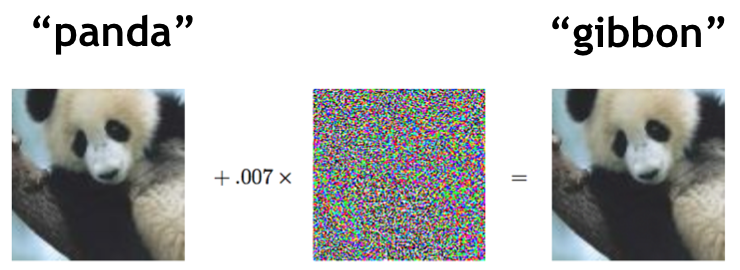
\includegraphics[width=0.6\linewidth]{panda}
\caption{Original image of a panda to which small and imperceptible to the human eye noise has been added, which caused misclassification of the image into a gibbon.}
\label{fig:panda}
\end{figure}

\subsection{Mathematical formulation}

Let's try to formulate adversarial examples more mathematically, from the perspective of optimization. Recall that our fundamental problem of supervised learning is to provide an accurate mapping from an input $x_i$ to an output $y_i$ by optimizing over some set of model parameters $\theta$. This can be formulated as a minimization problem

\begin{align*}
\min_\theta \text{loss}(\theta, x_i, y_i)
\end{align*}

This minimization problem is solved by running an iterative gradient descent algorithm over continuously differentiable model parameters.

The above approach has been the workhorse of supervised learning this decade. However, it only takes a small tweak to this optimization paradigm to find adversarial examples. To execute an adversarial attack, we take our model parameters $\theta$ as fixed and instead optimize over our \textit{inputs}. More specifically, we search for a perturbation $\delta$ that can be added to $x_i$ to \textit{maximize} the resulting model loss:

\begin{align*}
\max_{\delta\in\Delta} \text{loss}(\theta, x_i + \delta, y_i)
\end{align*}

If $\delta$ is unconstrained, an attack could be taken as the difference between one class and another. However, this wouldn't be rightfully considered as an adversarial example. 
%this optimization process could alter the image enough to actually change the true label class $y_i$, and this wouldn't be rightfully considered an adversarial example. 
As such, we constrain the $\delta$ to be from a class of appropriate perturbations $\Delta$.

The choice of how to define $\Delta$ is very domain-specific and should thus be chosen after carefully considering the problem at hand. Common approaches include:

%(TODO: fill in from slides)
\begin{itemize}
  \item Norm bound: none of the pixels are perturbed by more than $\epsilon$, i.e. $||\delta|| \leq \epsilon$, most commonly $L_2$ or $L_\infty$ 
  \item VGG similarity: cosine similarity between models
  \item Rotations and translations
\end{itemize}

For the purpose of this class, we will generally assume that $\Delta = ||\delta||_\infty \leq \epsilon$.


\section{Properties of Adversarial Examples}

\subsection{Adversarial examples (probably) arise from linearities}

Adversarial examples have been shown to exist for every class of machine learning models ever tested, including simple single-layer models. To see why even simple linear models are susceptible to adversarial attacks, consider the simplest model.

\begin{align*}
f(x) = w^Tx
\end{align*}

If we apply a small adversarial perturbation to this model, we have

\begin{align*}
f(x) = w^T(x + \delta) \\
= w^Tx + w^T\delta
\end{align*}

To maximize the effect of this small perturbation we set $\delta_i = -\text{sign}(w_i)\epsilon$, then

\begin{align*}
= w^Tx + \epsilon|w|_1
\end{align*}

In the case that $w$ has high dimensionality, the small perturbation can be magnified by applying a bias in the direction away from this image's true class.

Finally, while deep neural networks possess many nonlinearities, they are \textit{piecewise linear} or locally linear.  As such, linear perturbations just like the above are thought to drive adversarial examples in deep networks \cite{goodfellow2014}.

\subsection{Adversarial examples are not random}

While it may be tempting to assume that adversarial examples are a product of the models poor robustness to random noise, empirical studies have demonstrated that this is not the case.  In fact, 
%[TODO - I CANT FIND THE PAPER WHERE THE FIGURE BELOW IS FROM-HELP?], 
adding random noise to the inputs produces adversarial examples a small fraction of the time (Figure \ref{fig:notnoise}), whereas adding noise in the direction of a calculated attack (the FGSM attack in this case, see below for details), adversarial examples abound (Figure \ref{fig:noise_res}).

\begin{figure}[!h]
\centering
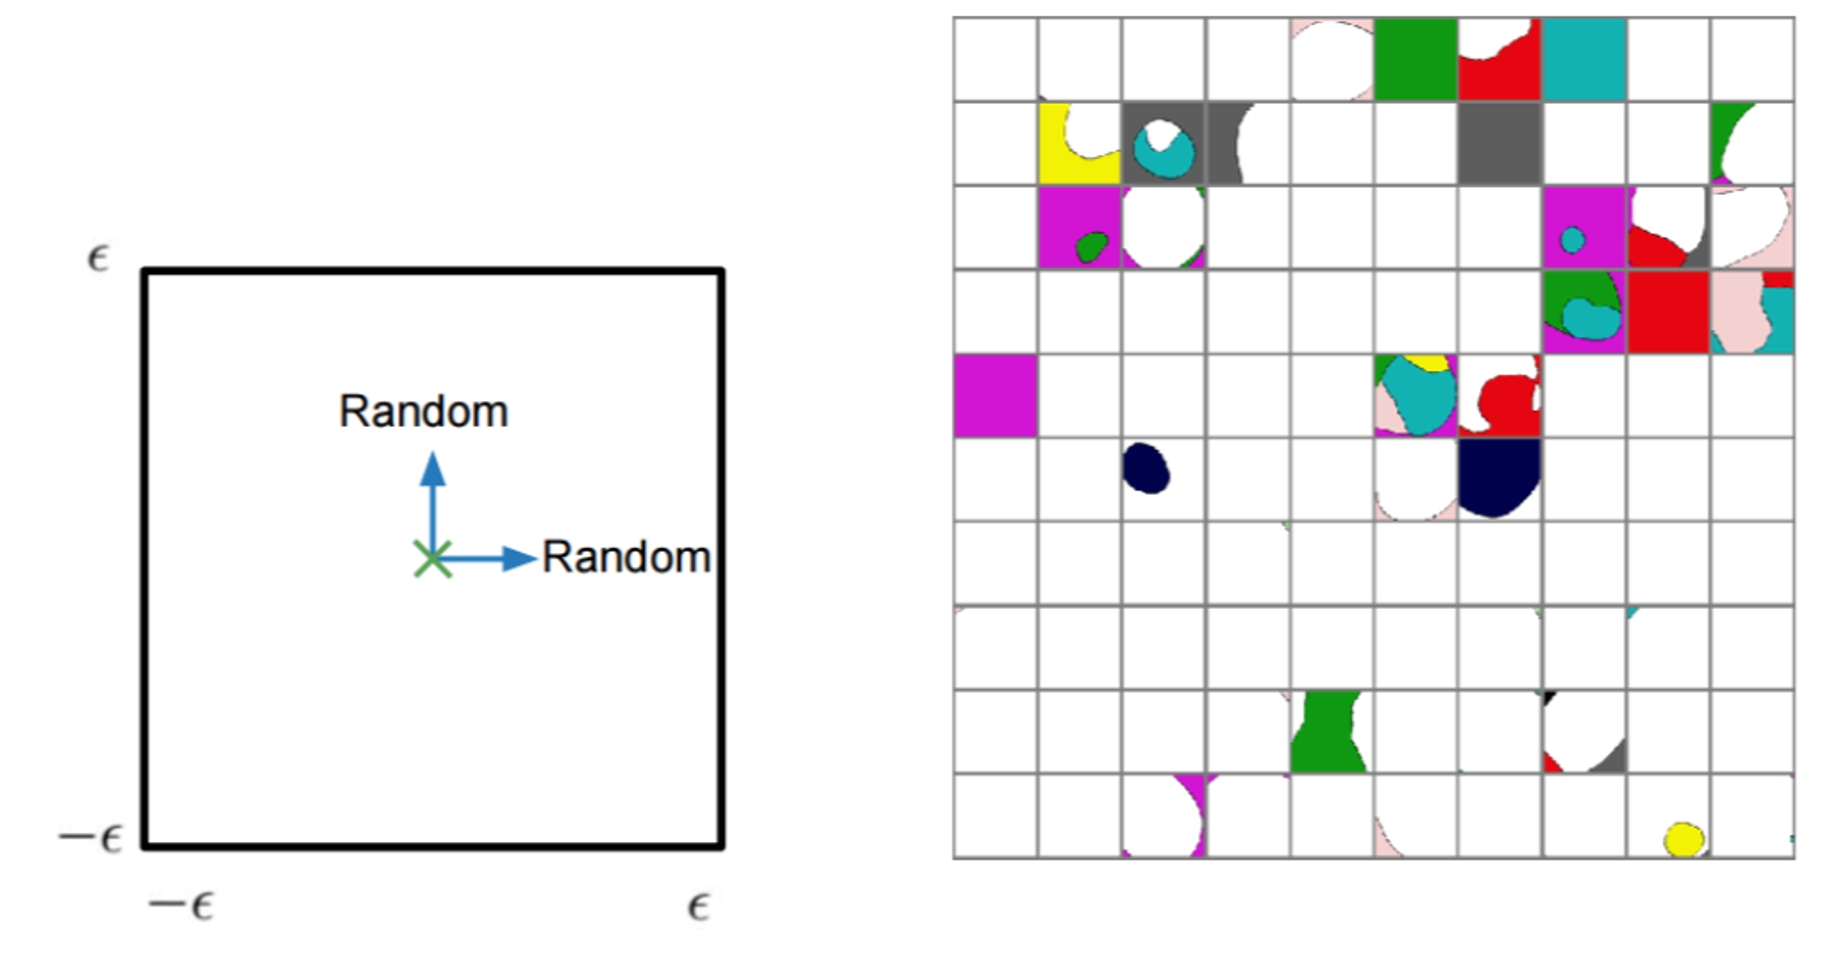
\includegraphics[width=0.5\linewidth]{notnoise}
\caption{Adversarial examples are not noise.}
\label{fig:notnoise}
\end{figure}

\begin{figure}[!h]
\centering
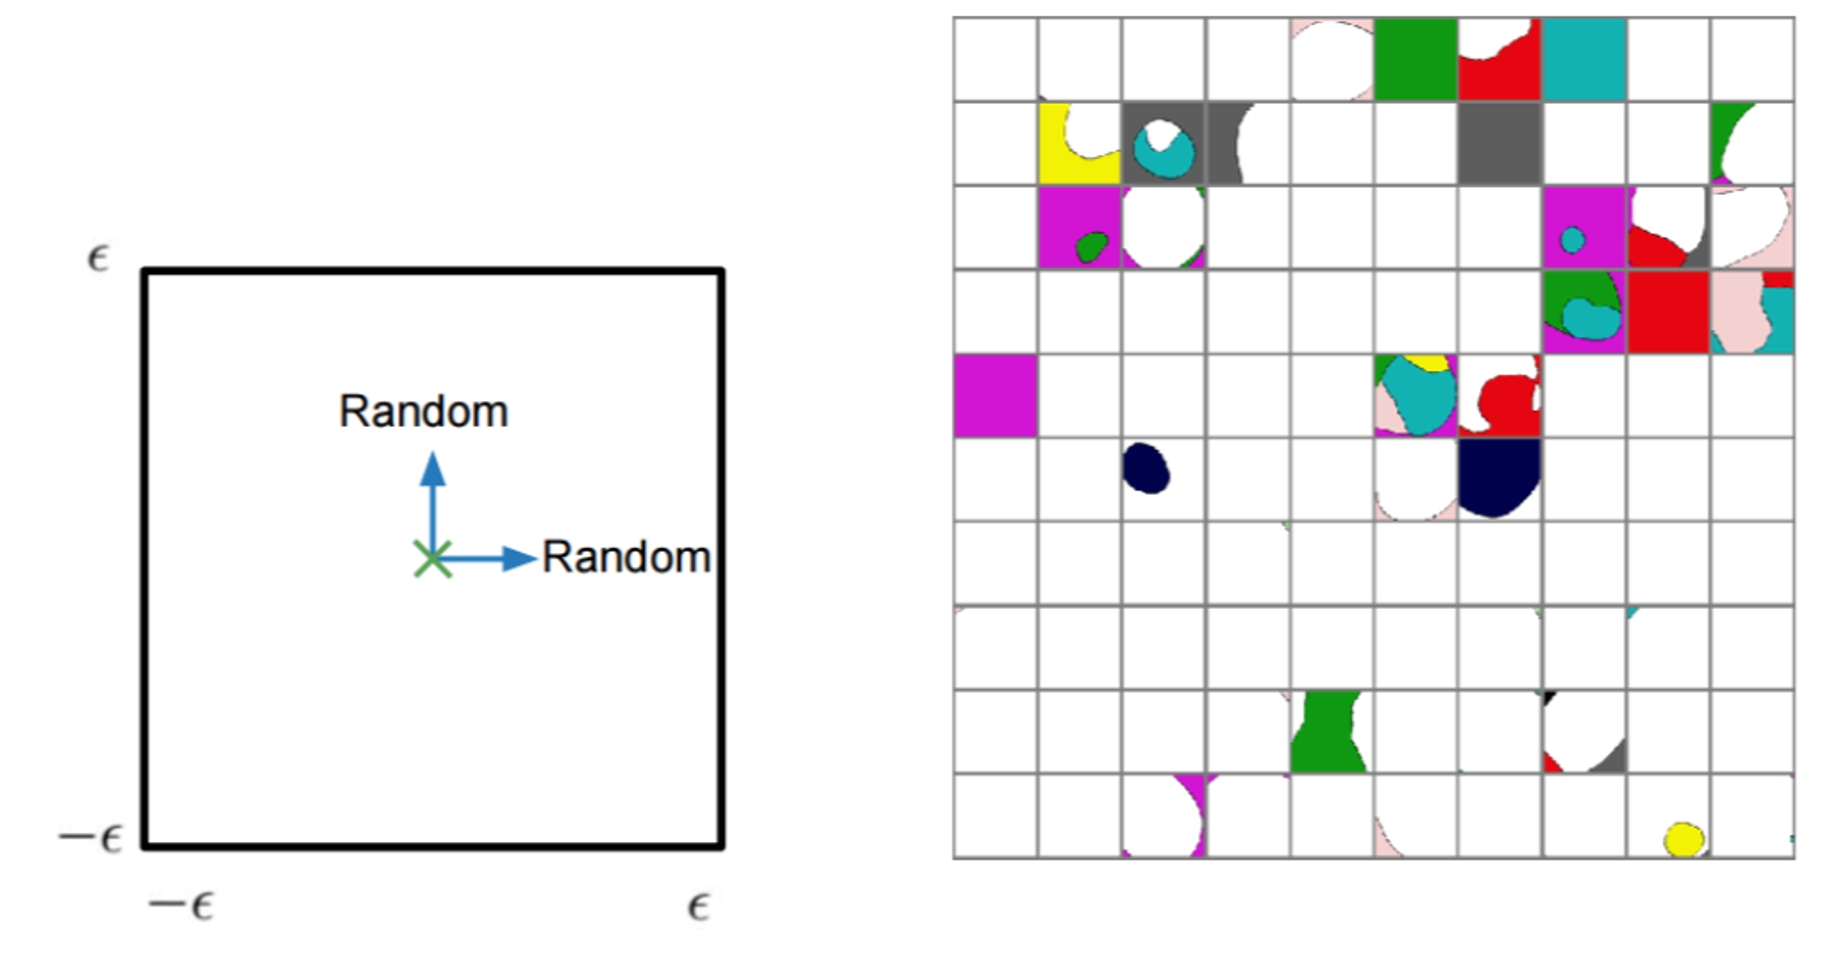
\includegraphics[width=0.5\linewidth]{notnoise}
\caption{Adversarial examples are noise-resistant.}
\label{fig:noise_res}
\end{figure}

Precisely how large is the space of adversarial examples?  Tramer et al. \cite{Tramer2017} sought to quantify the dimensionality of the adversarial subspaces. They found that only approximately 50 directions were adversarial (Figure \ref{fig:dimension}).
\begin{figure}[!h]
\centering
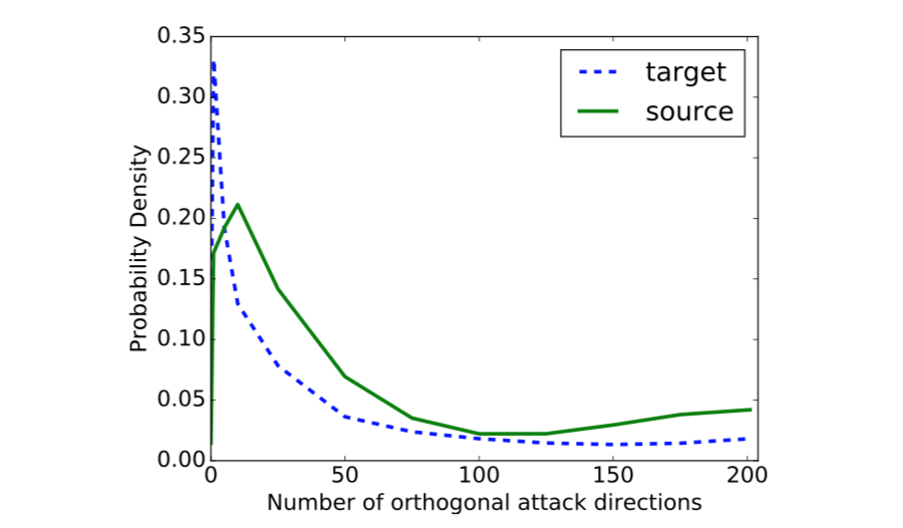
\includegraphics[width=0.5\linewidth]{dimension}
\caption{Number of successful orthogonal adversarial perturbations on the source DNN model and of the number of perturbations that transfer to the target DNN model.}
\label{fig:dimension}
\end{figure}

Despite the comparatively small dimensionality of the adversarial subspaces, however, other studies have shown that models can be "wrong almost everywhere." \cite{goodfellow2014}. In other words, if you choose \textit{random} inputs to the neural network, you can still perturb the images into any any class you desire in most cases (Figure \ref{fig:modelsarewrong}).

\begin{figure}[!h]
\centering
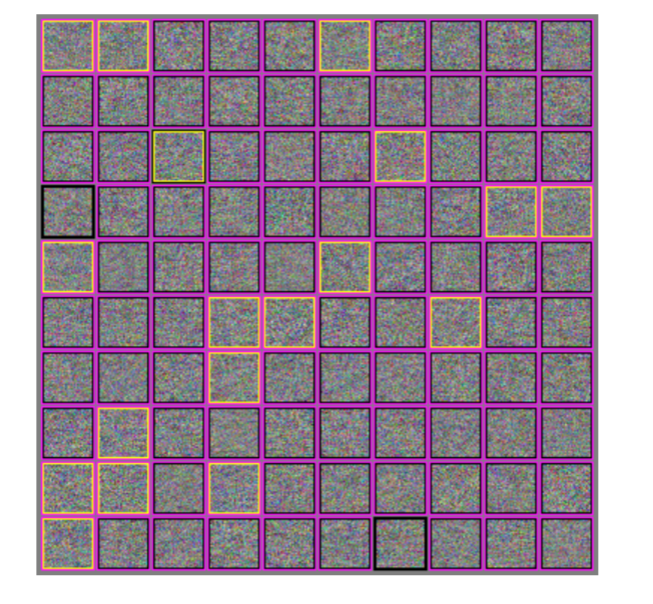
\includegraphics[width=0.5\linewidth]{modelsarewrong}
\caption{Randomly generated fooling images for a convolutional network trained on CIFAR-10. These examples were generated by drawing a sample from an isotropic Gaussian, then taking a gradient sign step in the direction that increases the probability of the airplane class. Yellow boxes indicate samples that successfully fool the model into believing an airplane is present with at least 50\% confidence.}
\label{fig:modelsarewrong}
\end{figure}

\subsection{A word of caution}

A cottage industry has sprung up generating various ad hoc defenses to specific adversarial attacks. Time and time again, these defenses have been repeatedly broken, often extremely quickly \cite{Athalye2018, Biggio2017}. \footnote{One example: Members of the Wagner lab at Berkeley recently broke 7/8 defenses presented at the most recent ICLR -- all within days of the conference!}  This often plays out as a rapid back-and-forth arms race between defense designers and defense breakers.

As such, while studying defenses for these attacks is very important, please don't add to the noise by blindly assuming you've solved this problem with another simple trick. Instead, study the literature and see what has been tried and consider how your idea might relate.


\section{A principled approach to avoiding adversarial examples}

\subsection{Why we shouldn't be surpised that adversarial examples arise from our typical formulations of supervised learning }

As we attempt to avoid adversarial examples, it is first important to note that the phenomenon as it currently exists does not necessarily demonstrate a \textit{failure} of machine learning models per se. Rather, adversarial examples reflect a disconnect between what we explicitly optimize our models to do and the behavior that we (often mistakenly) expect our models to implicitly learn along the way.

To make this statement more precise, let's consider the problem we generally hope to solve in supervised learning from a statistical perspective. In learning our model, we generally seek to minimize our expected model loss over the true data distribution $(x,y)~\mathcal{D}$:

\begin{align*}
\min_{\theta} E_{(x,y) \sim \mathcal{D}} \big[\text{loss}(\theta, x, y) \big] 
\end{align*}

Likewise, our training procedure can be framed as seeking to approximate this true minimum expected loss by finding the minimum empirical loss over the training data:

\begin{align*}
\min_{\theta} \hat{E} \big[\text{loss}(\theta, x_i, y_i) \big] 
\end{align*}

Both of the formulations above are designed to solve exactly the task of loss minimization and neither of the above formulations explicitly account for adversarial examples. Thus, requiring that the system is robust to adversarial examples, which as we saw are not random perturbations (they are essentially measure zero) is completely orthogonal to the empirical minimization problem above. Since, we never asked our machine learning algorithm not to have adversarial examples, we should not be surprised to find adversarial examples

%which as we saw above represent a tiny subspace of the image distribution and thus almost certainly account for measure zero in the above expectations. As such, we shouldn't be surprised that models trained through the above framework.


\subsection{Towards a paradigm for adversarially robust generalization}
Once an understanding has been established of the task that our machine learning algorithm is solving and not solving, we can redefine our machine learning optimization task to suit our particular goals. Specifically, we can build supervised learning models that are robust to adversarial examples by modifying our learning problem to account for adversarial perturbations. This can be achieved by finding parameters $\theta$ that minimize the adversarial loss, which is the highest loss of a given data point after a perturbation $\delta$ out of all allowed perturbations $\Delta$:

\begin{align*}
\min_{\theta} E_{(x,y) \sim \mathcal{D}} \big[\max_{\delta\in\Delta} \text{loss}(\theta, x + \delta, y) \big] 
\end{align*}

%Instead of feeding samples from the distribution D directly into the loss L, we allow the adversary
%to perturb the input first.maximization problem aims to
%find an adversarial version of a given data point x that achieves a high loss

%This is precisely the problem of attacking a given neural network. On the other hand, the goal of the outer minimization problem is to find model parameters so that the “adversarial loss” given by the inner attack problemis minimized. This is precisely the problem of training a robust classifier using adversarial training techniques


%if we sample an example from a distribution, then I not only care how the example is classified itself but 
%take a maximum over all possible allowed perturbations and 

%then we have a guarantee

In order to solve the optimization problem posed above, we can perform \textit{adversarial training} \cite{Madry2017} (not to be confused with GANs) on the empirical loss:

\begin{align*}
\min_{\theta} \frac{1}{m} \hat{E} \big[\max_{\delta\in\Delta} \text{loss}(\theta, x_i + \delta, y_i) \big] 
\end{align*}

%In short, this approach is to perform data augmentation in the adversarial directions.


The adversarial training can be performed via alternating steps, by first solving the maximization problem, which is exactly solving the attack problem via your method of choice, and then taking the gradient with respect to our redefined notion of loss as the adversarial loss:

\begin{align*}
\text{lossadv}(\theta, x_i + \delta, y_i) =  \max_{\delta\in\Delta} \text{loss}(\theta, x_i + \delta, y_i)
\end{align*}

For each model parameter update: a batch of images is subsampled, the worst case perturbation for each of the images is found and gradient descent is computed on the perturbed image to update model parameters. This solution to the adversarial learning problem should not be confused with GANs. Instead, this approach is akin to data augmentation, where the model is trained not on the data itself but on modified data and in this particular case, adversarially modified data. More generally, data augmentation can be thought of as replacing the max in the training equation above with an expectation over random perturbation.

Although the formulation above is non-convex, we hope that our deep learning methods for solving highly non-convex problems will perform well for this task.

\section{Adversarial Attacks}

The adversarial problem boils down to finding the optimal direction to move within the box of radius $\delta$ surrounding each input $x_i$ that will maximize the probability the model assigns to an incorrect class.  Single-step and iterative approaches have been proposed \cite{Madry2017}.

\begin{figure}[!h]
\centering
\begin{subfigure}[t]{0.45\textwidth}
\centerline{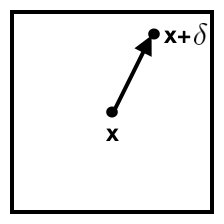
\includegraphics[width=0.5\linewidth]{fgsm.png}}
\caption{Fast Gradient Sign Method (FGSM)}
\label{fig:fgsm}
\end{subfigure}
\centering
\begin{subfigure}[t]{0.45\textwidth}
\centerline{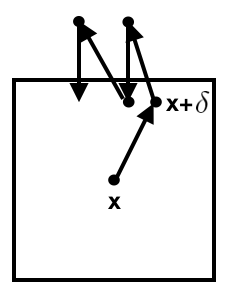
\includegraphics[width=0.5\linewidth]{pgd.png}}
\caption{Projected Gradient Descent (PGD)}
\label{fig:pgd}
\end{subfigure}
\caption{Gradient updates for FGSM (a) vs. PGD (b) where $x$ is the training example, the box is the space of perturbations and $\delta$ is a particular perturbation.}
\end{figure}


\subsection{Fast Gradient Sign Method (FGSM)}

The fast gradient sign method (FGSM) (Figure \ref{fig:fgsm}) was the first general adversarial attack proposed and represents the optimal single step attack. 

\begin{align*}
\delta = \eta \nabla_x \text{loss}(\theta, x_i, y_i)
\end{align*}

In this case, the set of perturbations is constrained such that $||\delta||_\infty\leq\epsilon$, resulting in the following gradient update:

\begin{align*}
\delta = \eta \nabla_x \text{sign}\Big(\text{loss}(\theta, x_i, y_i)\Big)
\end{align*}

This attack allows us to generate a set of images that are adversarial for the parameters of this network. particular training example. The fact that this method can find adversarial examples in complex neural networks suggests that these models are stepwise linear.

\subsection{Projected Gradient Descent Methods (PGD)}

Projected Gradient Descent (PGD) methods involves using FGSM with multiple steps. Additionally, we constrain the perturbation to within the permitted box around $x_i$. To ensure this, each time PGD takes a step, it checks if it has moved out of the box, and applies a projection back into the box if necessary (Figure \ref{fig:pgd}).
%[TODO: consider writing in algorithm form?]
PGD is naturally more expensive than FGSM, but allows for more effective attacks.

\section{Properties of adversarial attacks}

Through experiments using MNIST and CIFAR10, the following properties of adversarial training have been observed \cite{Madry2017}:
\begin{itemize}
\item The choice of the attack method is important
\item The loss of the final solution is a well-concentrated distribution
\item Model capacity matters
\end{itemize}

Comparison of FGSM vs. PGD revealed that PGD results in much better performance than FGSM (Figure \ref{fig:pgd_fgsm}), which linearizes the inner maximization problem.
\begin{figure}[!h]
\centering
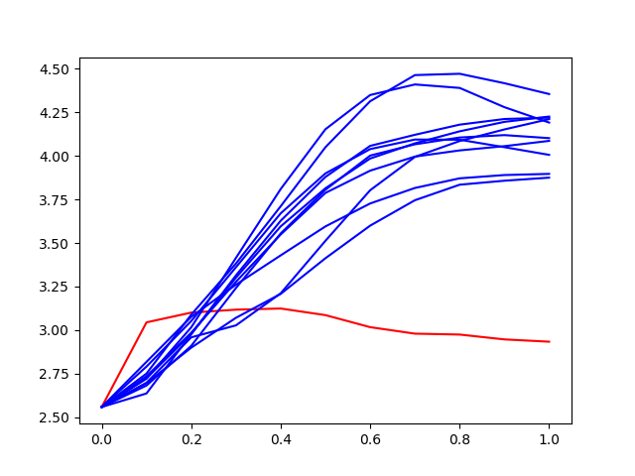
\includegraphics[width=0.5\linewidth]{pgd_fgsm}
\caption{The choice of attack method - FGSM (red) vs. PGD (blue) matters.}
\label{fig:pgd_fgsm}
\end{figure}

Since PGD solves a non-convex problem, the solution given by PGD is one of possible local maxima. However, it is possible that much larger local maxima exist that PGD is unable to find. Madry et al. have investigated this behavior by performing many restarts. As shown in Figure \ref{fig:local_maxima}, the final loss follows a well-concentrated distribution.

\begin{figure}[!h]
\centering
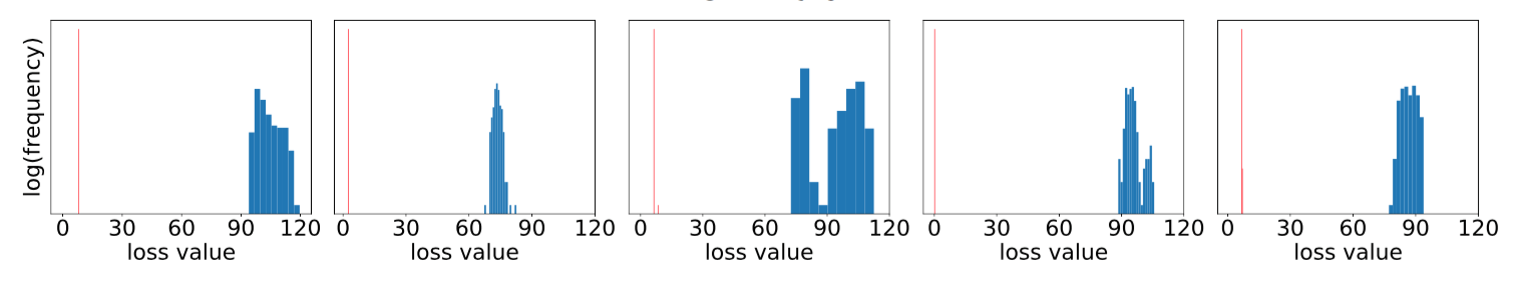
\includegraphics[width=0.9\linewidth]{dist_local_maxima}
\caption{Values of the local maxima given by the cross-entropy loss for five examples from the
MNIST and CIFAR10 evaluation datasets. For each example, PGD is started uniformly at random around the example and iterated until the loss plateaus.The blue histogram corresponds to the loss on a naturally trained network, while
the red histogram corresponds to the adversarially trained counterpart. The loss is significantly
smaller for the adversarially trained networks, and the final loss values are very concentrated without
any outliers.}
\label{fig:local_maxima}
\end{figure}

Training against strong adversarial examples requires a stronger classifier with more capacity to distribguish one class from another. Figure \ref{fig:boundary} shows that a simple linear decision boundary is unable to seprate all adversarial examples within $\ell_{\infty}$ of the training point because it is not complex enough. However, when a more complicated decision boundary can be learned, smaller number of adversarial examples will be misclassified. 
\begin{figure}[!h]
\centering
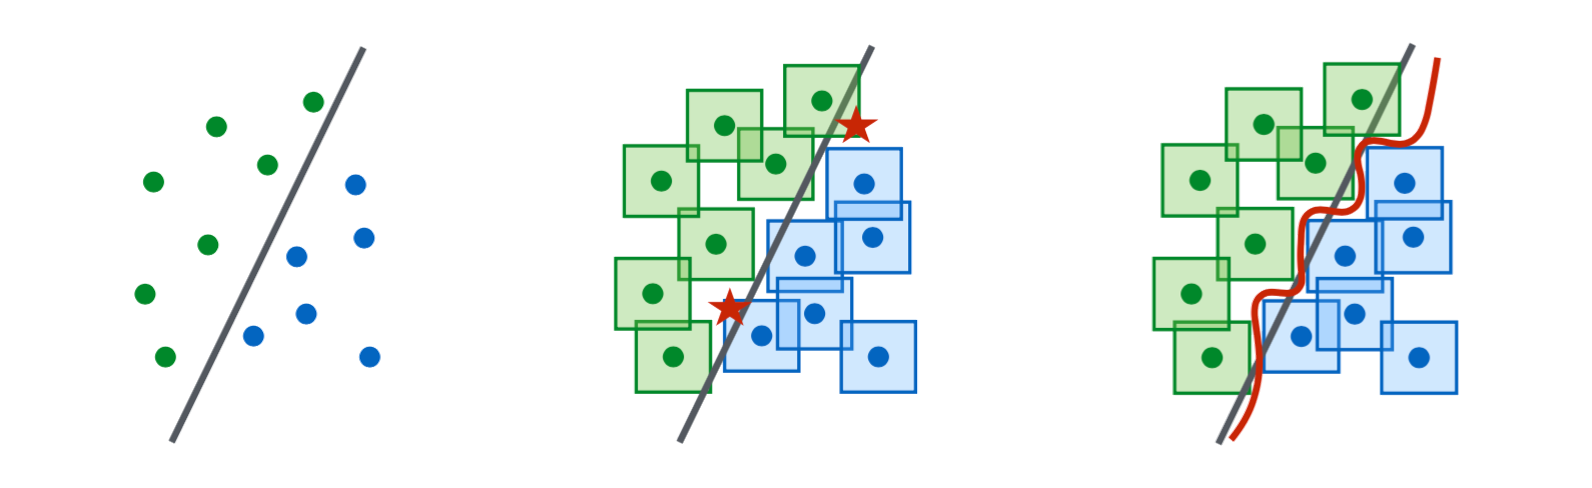
\includegraphics[width=0.9\linewidth]{boundary}
\caption{Natural classification (left) vs. adversarial boundaries (right) corresponding to $\ell_{\infty}$ ball around training points.}
\label{fig:boundary}
\end{figure}

This intuition has been captured via experimental results that trained convolutional
networks on natural examples, FGSM examples and PGD examples while doubling the size
of network. As shown in Figure \ref{fig:capacity}, small capacity networks have larger loss even on natural examples, indicating that capacity alone increases accuracy. When adversaries like PGD are added, for small capacity networks PGD fails to learn a meaningful decision boundary and performance is sacrificed for robustness. On the other hand, for large capacity networks a robust and accurate solution can be achieved with PGD adversary.

\begin{figure}[!h]
\centering
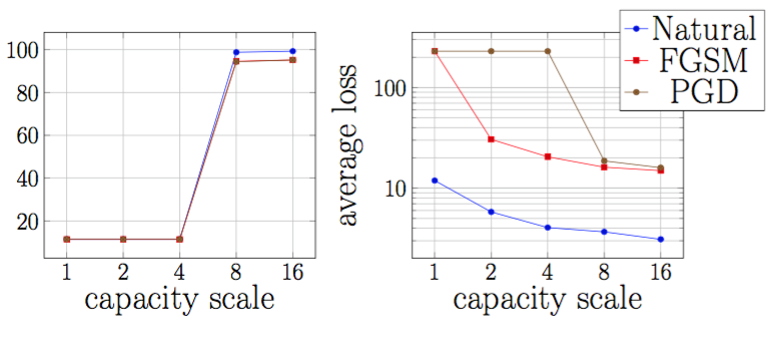
\includegraphics[width=0.6\linewidth]{capacity}
\caption{Average accuracy and average loss vs. capacity of convolutional neural networks trained with natural examples, FGSM adversary and PGD adversary.}
\label{fig:capacity}
\end{figure}


The PGD adversary was trained for both MNIST and CIFAR10 and it has been shown that there is a steady decrease in the training loss of
adversarial examples (Figure \ref{fig:itworks}) showing an indication that the original adversarial training optimization problem is indeed being solved during training.

\begin{figure}[!h]
\centering
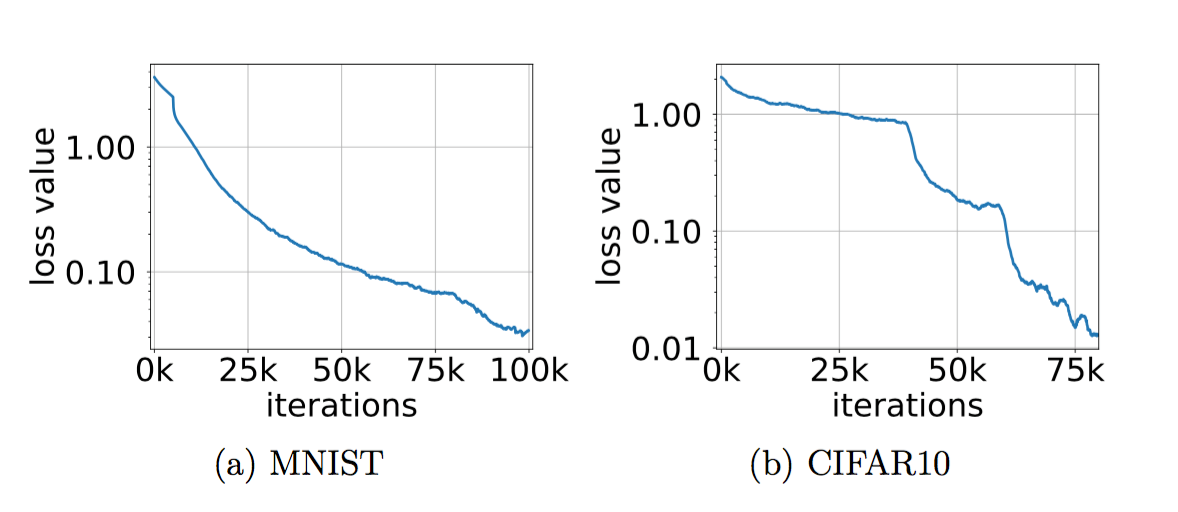
\includegraphics[width=0.6\linewidth]{itworks}
\caption{Value of adversarial loss function on MNIST and CIFAR10 datasets during training.}
\label{fig:itworks}
\end{figure}

\section{Conclusions}

Deep learning models are susceptible to adversarial examples where the differences between training and adversarial images are indistinguishable to the human eye. It has been shown that adversarial examples are not random noise, but are a subspace of perturbations. A variety of approaches that come up with new attack and defense methods have been coming out. Recently a new paradigm that explicitly optimizes for robustness to attacks has been developed. 


\bibliographystyle{abbrv}
\bibliography{bib}

\end{document}

